\begin{figure*}[h!]
    \centering
    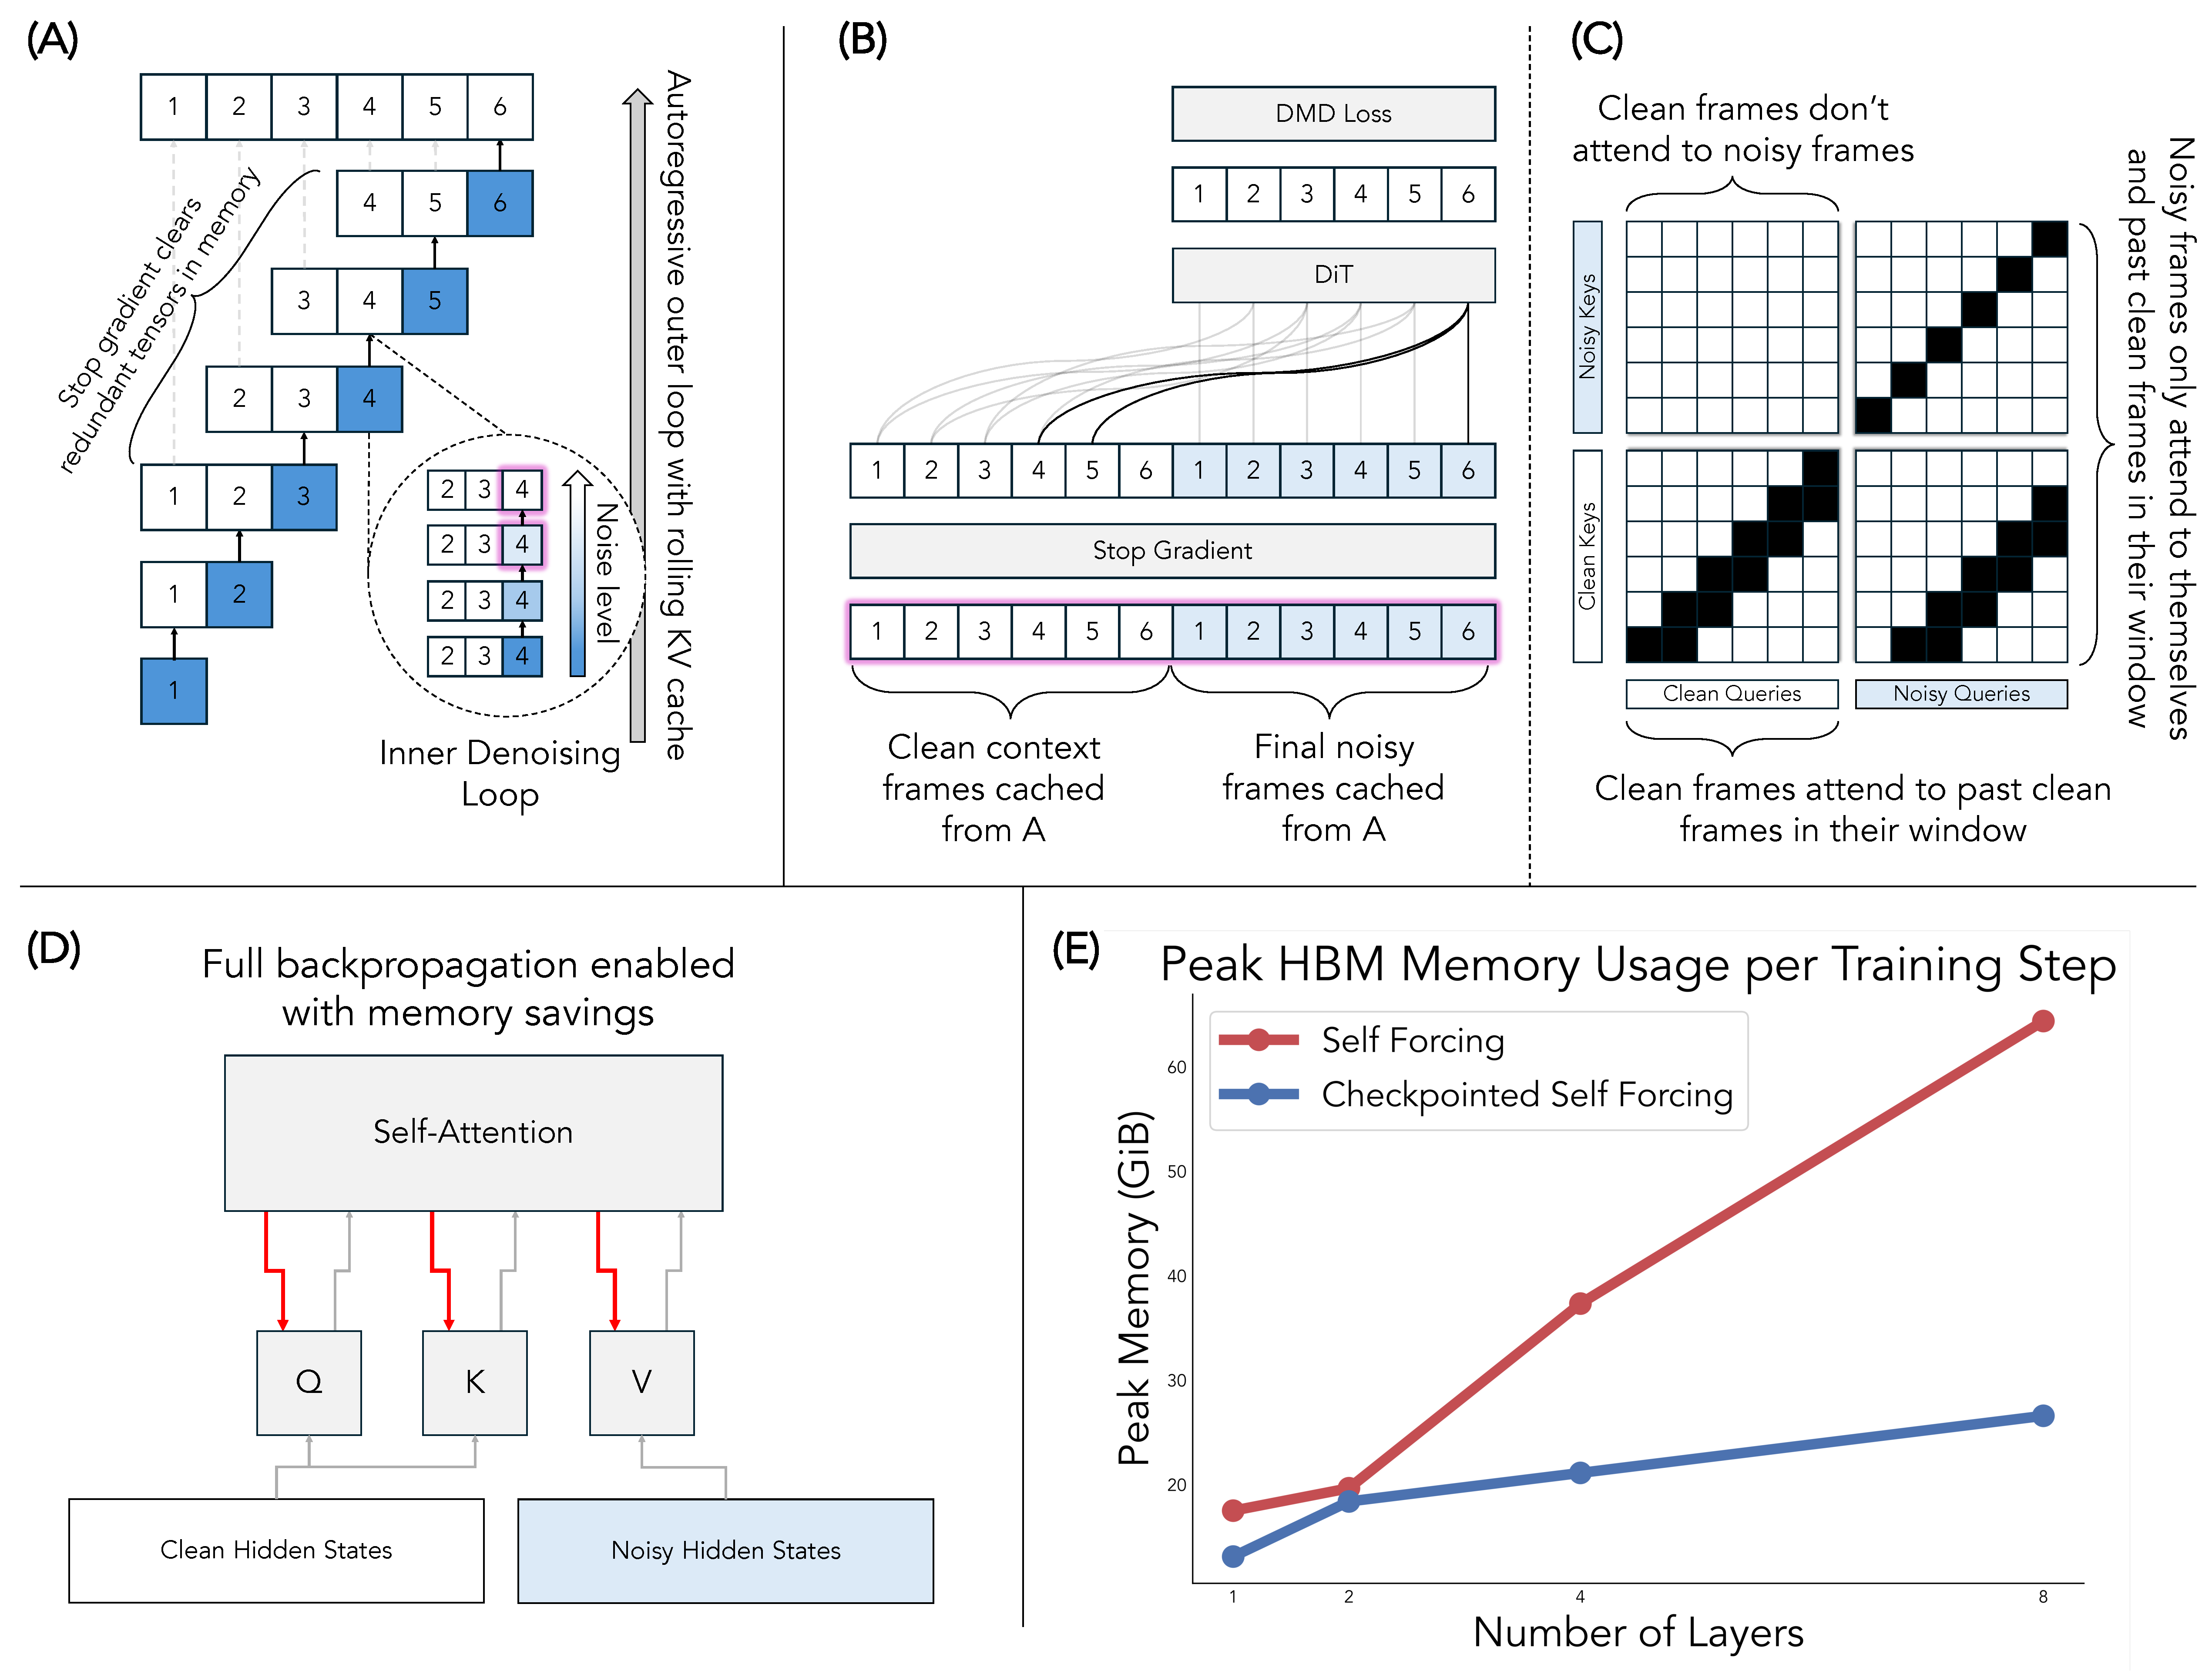
\includegraphics[width=\linewidth]{figs/assets/sf.pdf}
    \caption{An overview of \oursf. \textbf{(A)} A video is generated with a sliding-window KV cache. The computation graph in Jax contains redundant tensors, making naive backpropagation memory prohibitive. \textbf{(B)} Our recomputation step simulates the last step of denoising for every frame in parallel. Clean context frames and final noisy frames are cached from the previous step. \textbf{(C)} An illustration of the attention mask used in part B (black squares denote attention). This attention mask allows us to simulate the final denoising step of the rollout in parallel. \textbf{(D)} Leveraging these memory savings, we enable backpropagation through KV layers (avoiding the standard stop-gradient of Self Forcing), which we show improves visual generation in~\cref{sec:experiments}. Specifically, we allow gradients to flow in line 29 of~\cref{alg:self_forcing_algorithms}. \textbf{(E)} Peak memory comparison between naive and \oursf across varying depths. Scaled-down networks are used to prevent OOM errors in the naive baseline. }
    \label{fig:self_forcing}
\end{figure*}
